\documentclass[aps,pra,preprint,superscriptaddress,nofootinbib]{revtex4-2}
\usepackage{amsmath}
\usepackage{amssymb}
\usepackage{tikz}
\usetikzlibrary{calc,arrows,decorations.pathmorphing,intersections}
\usepackage{pgfplots}
\pgfplotsset{width=10cm,compat=1.15}
\usepgfplotslibrary{fillbetween}
\usepackage[T1]{fontenc}
\usepackage{color}

\begin{document}

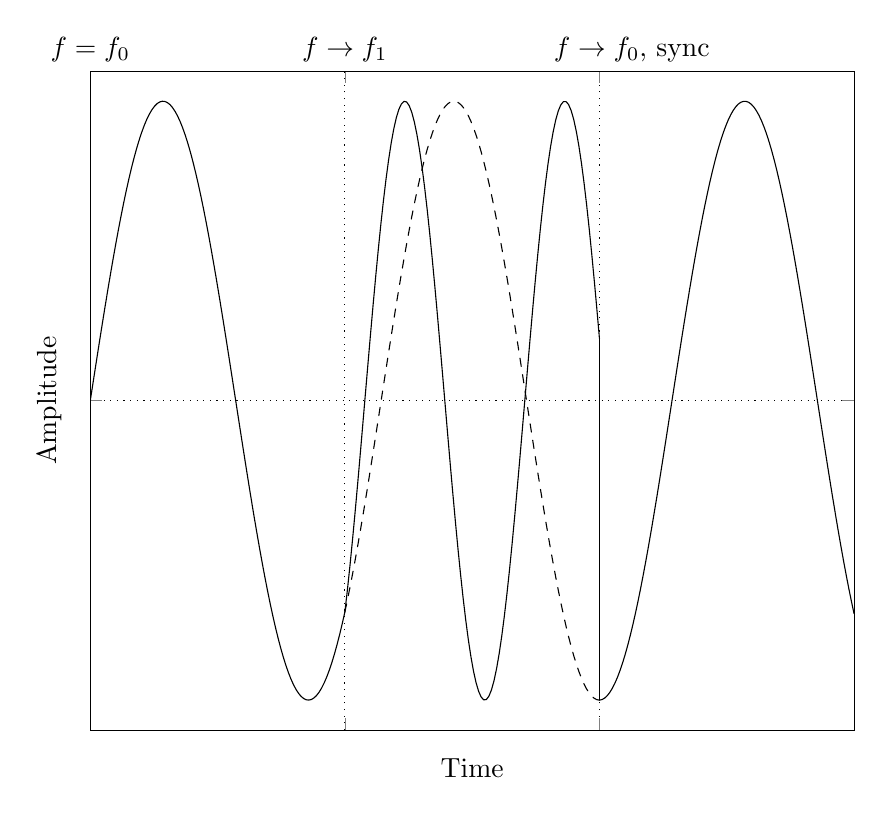
\begin{tikzpicture}
		\pgfplotsset{
			scale only axis,
                        major grid style={dotted,black},
			xmin=0.0,xmax=3.0,
			ymin=-1.1,ymax=1.1,
            every axis plot/.append style={line join=round,line cap=round,clip=false}
		}

		\begin{axis}[
                        width=0.8\linewidth,
			tick style={grid=major},
			% xlabel=Time, 
			ylabel=Amplitude,
			samples=100,
                        xticklabels={$f=f_0$,$f\rightarrow f_1$,\qquad~$f\rightarrow f_0\text{, sync}$,},
                        xtick={0,1,2,3},
			axis x line*=top,
                        ytick={-2,0,2},
                        yticklabels={,,}
			]
        \addplot[draw=black,dashed][domain = 1:2]{sin(5.5*deg(x))};
        \addplot[][domain = 0:1]{sin(5.5*deg(x))};
        \addplot[][domain = 1:2]{sin(10.0*deg(x-1)+5.5*deg(1.0))};
        \addplot[][domain = 2:3]{sin(5.5*deg(x)};
        \addplot[draw=black] coordinates {(2.0,{sin(5.5*deg(2.0)}) (2.0,{sin(10.0*deg(1)+5.5*deg(1.0))})};
        \end{axis}
        \begin{axis}[
                width=0.8\linewidth,
	        xlabel=Time,
	        xmin=0.0,xmax=3.0,
		ymin=-1.1,ymax=1.1,
		xtick={0,1,2,3},
                xticklabels={,,,},
                ytick={-2,0,2},
                yticklabels={,,}
		]
	\end{axis}
\end{tikzpicture}

\end{document}